% SPDX-FileCopyrightText: © 2026 Idiap Research Institute <contact@idiap.ch>
%
% SPDX-FileContributor: Andre Freitas <andre.freitas@idiap.ch>
% Neuro-symbolic AI Group
%
% SPDX-FileContributor: Danilo Gusicuma <danilo.gusicuma@idiap.ch>
% Neuro-symbolic AI Group
%
% SPDX-License-Identifier: MIT
\section{Introduction: what makes a problem require new concepts?}
\label{sec:conceptual-introduction}
A difficult problem can persist even when individual calculations are correct.
The difficulty may lie in what the calculation is about: which objects count as
the same, which distinctions a representation preserves, what an explanation is
expected to unify, or which assumptions make a question meaningful. An inquiry
then needs to examine its conceptual commitments as well as derive consequences
from them. The question organizing this paper is:
\begin{quote}
How does a scientific inquiry locate a tension in its current understanding,
transform the concepts responsible for it, and turn that transformation into
more precise questions and obligations?
\end{quote}

We develop an interpretive account of source-prescribed reasoning procedures in
the Abducer repository. Their conceptual-discovery routes reconstruct an incumbent
framework, identify explanatory pressures, develop rivals, expose them to opposed
reflection, and retain what survives with its remaining burdens. Nineteen native
Prism workflow descriptions provide a complementary account of their typed
interfaces. These two sources describe different levels of organization. A
conceptual procedure explains why a change in understanding is sought; an
inferential classification identifies a kind of local move; a typed interface
records the information that the move consumes and produces.

Our central proposal is to organize the account around changes in the conceptual
situation. These include recognizing an inadequate distinction, diagnosing its
origin, constructing a mediator, challenging its consequences, and revising the
question itself. Such changes can combine several inferential operations. Calling
the construction of a mediator ``abduction'' leaves unanswered what tension it
addresses, what the mediator preserves, and why it introduces a new proof burden.
Those are the explanatory questions the main text follows.

A small constructed example will run through the discussion. Suppose a state is
represented by a pair $(x,y)$, but the modeled instantaneous observations depend only on
$q=x-y$, which is itself observable. Simultaneously translating both coordinates leaves every stipulated
instantaneous observation unchanged. Whether that identification also preserves
observable futures remains to be checked. A distance on raw pairs nevertheless treats translated
representatives as different states. The pressure is to reconcile the chosen
identity conditions with the intended observable question. This is an abstract
representation problem, not a model of a particular physical theory.

The contribution has three parts: an account of how conceptual pressures become
revisable commitments; a worked transformation showing both what a new
representation resolves and what it leaves open; and a supporting correspondence
to inferential operations and Prism interfaces. The appendices retain the formal
calculus and detailed explanations of all 65 declared occurrences in the nineteen
workflows. The examples illustrate the account; neither the source instructions
nor their exposition establish that a runtime realizes it or improves scientific
discovery.

\section{Reconstruct the situation and locate its tensions}
\label{sec:conceptual-situation}
Finding a tension starts with reconstructing what the current framework is
committed to. The source procedures ask for its primitives, identity conditions,
relations, mechanisms, inherited representation choices and explanatory ideals.
They also ask which successes a replacement must preserve. Without that second
part, it is easy to make a problem disappear by discarding the very phenomena or
constraints that made it scientifically significant.

An effective reconstruction connects each commitment to its role. Which
observations require a distinction? Which inference uses an assumption? Which
quantity is supposed to be invariant? Which result has been established only in a
restricted regime? A list of definitions is insufficient: the investigator needs
to see where commitments jointly constrain the same explanation. A failed
argument, a counterexample or a newly assimilated source can expose that point.
Conversely, a source that repeats a known result may leave the conceptual picture
unchanged; the procedures permit a justified finding of no change.

A conceptual tension is not necessarily a formal contradiction. It can be a
conflict between explanatory demands, a representation that loses a relevant
distinction, or a gap between local success and the scope of a proposed claim.
The following distinctions are an expository organization of such pressures,
not a complete taxonomy supplied by the native language.

\begin{table}[htbp]
\centering\small
\begin{tabularx}{\linewidth}{@{}>{\raggedright\arraybackslash}p{.23\linewidth}>{\raggedright\arraybackslash}X>{\raggedright\arraybackslash}X@{}}
\toprule
Pressure & What brings it into view & What must be investigated \\
\midrule
Incompatible commitments & Two premises cannot hold together in the stated domain & Which premise or domain restriction should change \\
Identity mismatch & A representation distinguishes objects the target treats as equivalent & Which equivalence and observables justify identifying them \\
Explanatory opacity & A calculation succeeds but the proposed mechanism explains no dependency & What mechanism would make the success intelligible \\
Transfer failure & A result works in one carrier or regime but its application lacks a bridge & Which structure and error control the transfer requires \\
Incomplete unification & A common description removes differences that matter to the target & Which mediator can connect the cases while retaining those differences \\
\bottomrule
\end{tabularx}
\caption{Ways a conceptual pressure can be localized. Each points to a different
investigation; none by itself establishes that a new ontology is needed.}
\label{tab:conceptual-pressures}
\end{table}

In the running example, $(1,0)$ and $(2,1)$ give the same $q=1$. Their nonzero
Euclidean separation is mathematically consistent. The tension arises only if raw
coordinate distance is used to express a notion of difference intended to depend
on the stipulated observations. If absolute position becomes observable, the two
pairs may genuinely need to remain distinct. The diagnosis therefore depends on
the target and its observable commitments, not merely on noticing a symmetry.

The immediate product is a localized pressure: a named commitment, the failure or
opacity it produces, the successes it must retain, and a question that could
change the diagnosis. This is already an advance over saying that a problem is
``hard.'' It tells later invention what needs changing and what must survive.

\section{Diagnose what kind of change is warranted}
\label{sec:conceptual-diagnosis}
The next question is whether the pressure comes from the concepts or from an
unfinished task within adequate concepts. The conceptual-discovery instructions
explicitly allow a nonconceptual diagnosis. A missing calculation should lead to
derivation; a missing premise proof to proof work; an unresolved empirical
distinction to a suitable observation. A new ontology is warranted neither by
the difficulty of the problem nor by the availability of an invention skill.

Diagnosis traces an attempted inference backward. At which use of an object,
identity condition, model or regime did the argument stop carrying its intended
meaning? Would a better estimate repair the step without changing those objects?
Does the desired transfer require an independently specified correspondence?
Would adding a premise merely assume the intended conclusion? These questions
separate local incompleteness from pressure to reorganize the representation.

For the pair representation, calculating the existing Euclidean distance more
accurately would not make it invariant under independent choices of equivalent
representatives. The difficulty concerns what counts as a state difference. But
if the target has already been correctly expressed in $q$ and the remaining task
is to solve a well-defined equation for $q$, more conceptual invention may add
nothing. The same research episode can therefore need conceptual revision at one
point and routine derivation at another.

Diagnosis is revisable. A purported representational defect may turn out to
reflect a real observable that the initial reconstruction omitted. A failed
calculation may instead reveal that its variables conceal two different regimes.
The diagram makes these return paths explicit. It depicts explanatory
dependencies and possible revisions, not a mandatory runtime sequence.

\begin{figure}[htbp]
\centering
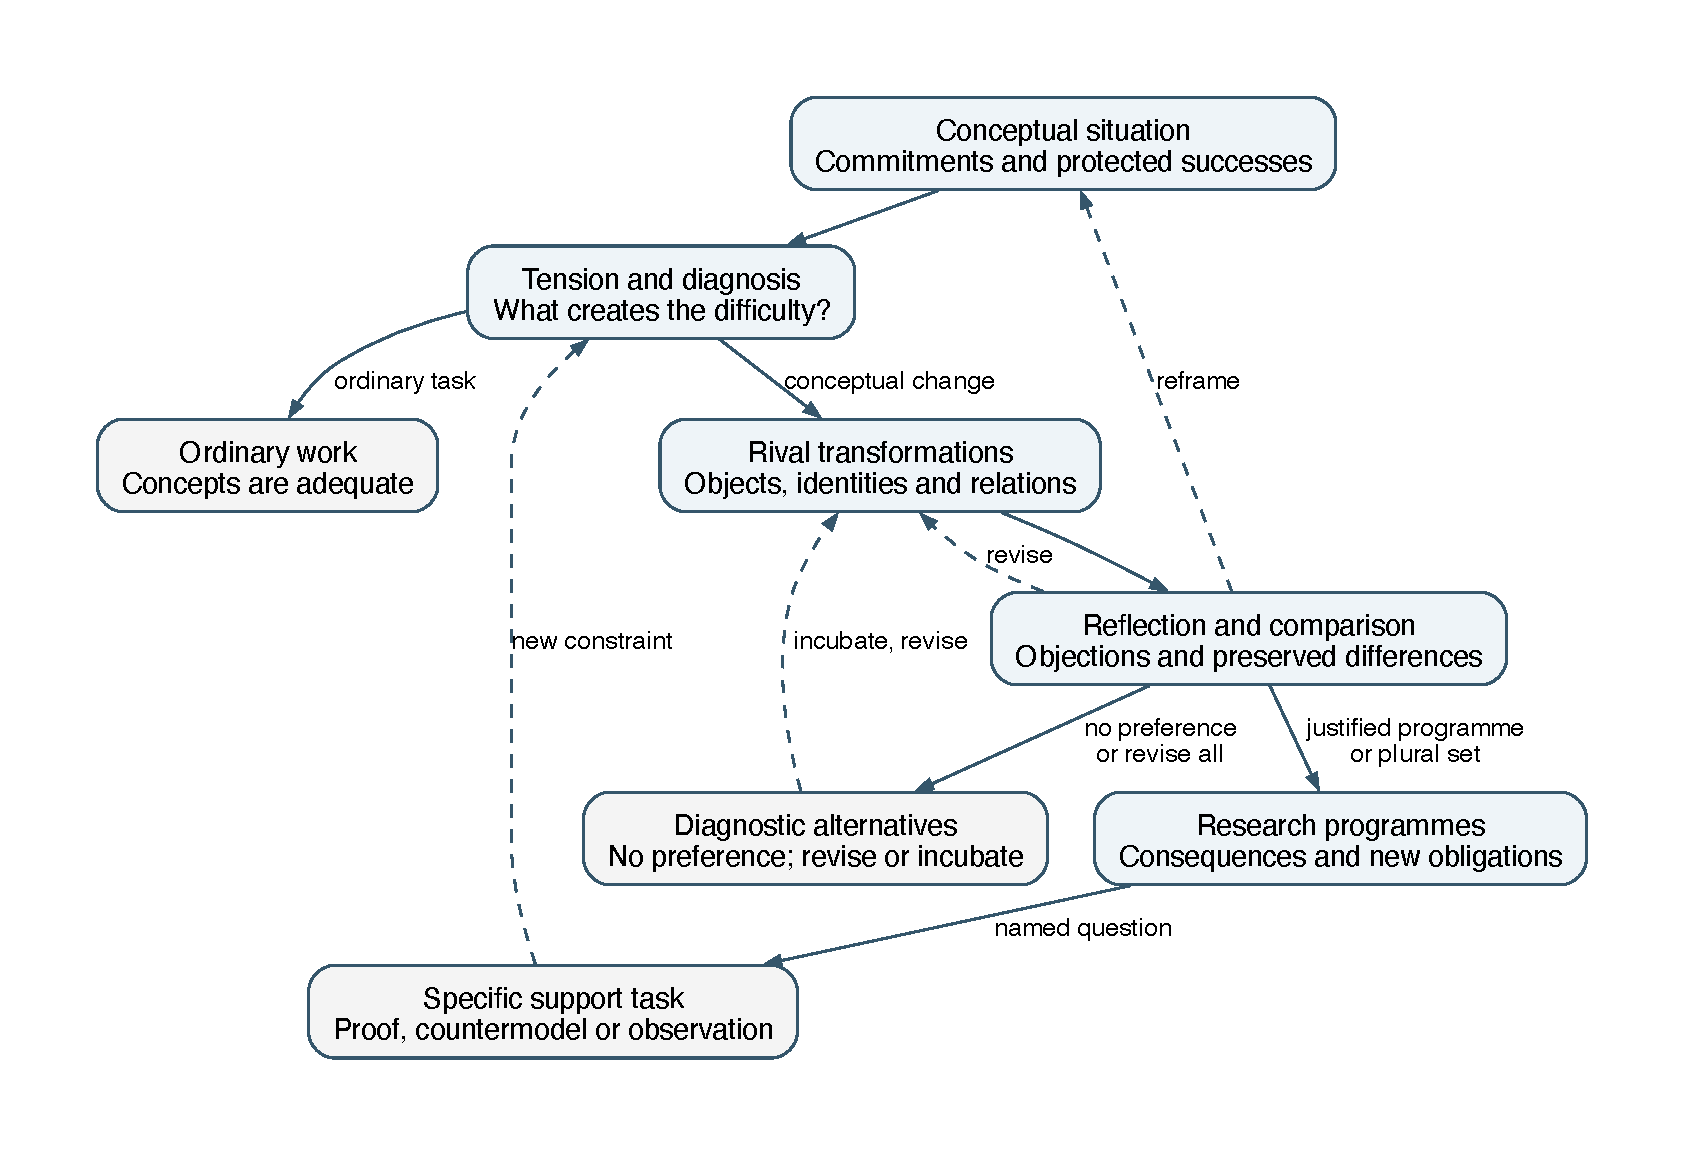
\includegraphics[width=\linewidth,height=.58\textheight,keepaspectratio]{paper-workflow-representations/conceptual-inquiry.pdf}
\caption{Conceptual inquiry organized by the question that changes next. Diagnosis
can send a task directly to derivation, reading or measurement. Alternative
construction and reflection can revise the original tension. A programme makes
remaining theoretical burdens explicit; support is requested when it can answer
a particular question. Alternatives without justified preference remain diagnostic
and do not authorize support investment. Solid arrows indicate possible information dependencies;
dashed arrows indicate revision. Neither style asserts native implementation.}
\label{fig:conceptual-inquiry}
\end{figure}

\section{Construct alternatives that change the explanatory commitments}
\label{sec:conceptual-alternatives}
Once a conceptual defect is localized, invention has an object. It may change a
primitive, an identity criterion, a relation, a causal dependency, a carrier or a
mediating map. The important distinction is between a changed conceptual system
and a new name for the incumbent one. A substantive alternative makes something
expressible or inferable that was previously obscured, or explains why a previous
question was misposed. It must also state which existing successes it retains.

The linked procedures preserve the incumbent as a rival, use literature and
negative knowledge to expose existing commitments and failed routes, and seek
materially different alternatives before attaching family labels. The number of
labels is not the number of conceptual alternatives. Proposals that differ only
in terminology belong to the same conceptual comparison; proposals with
incompatible mechanisms may need separate development even when they fit the same
observations. Detailed search and evaluation requirements differ by source
profile and are retained in the workflow appendix.

In the running example, one option is to use equivalence classes under simultaneous
translation as the state carrier. Another is to select a representative, for
example by setting $y=0$, and work with the remaining coordinate. A third is to
retain the redundant pair but restrict claims to invariant quantities. These are
different presentation and reasoning choices; they are not automatically three
different physical theories. Their relationship must itself be checked.

For each alternative the conceptual work includes specifying what changes, why it
addresses the pressure, what observations survive, and what could invalidate it.
Quotienting removes dependence on the redundant common translation, but now any
proposed dynamics must be compatible with that identification. Selecting a
representative can simplify calculations, but requires a justification that
representative choice does not alter the result. Retaining redundant coordinates
preserves convenient structure, but requires invariant statements throughout.
Each option reorganizes the burden rather than making it disappear.

An immature proposal can remain under development. It need not be sent immediately
to a proof engine or an experiment simply to obtain a status. However, incubation
must retain correction conditions: what would show that the new distinction is
irrelevant, that an established success was lost, or that the proposed mediator
merely defines the desired conclusion into existence?

\section{Deepen the alternatives through substantive reflection}
\label{sec:conceptual-reflection}
Reflection examines the commitments of a conceptual system, including the
investigator's reasons for preferring it. Its contribution is visible when an
identity condition changes, an objection narrows a claim, two alternatives split,
or a proposed synthesis creates a new burden. A repeated description of the same
candidate does not count as conceptual revision.

The conceptual-frontier source specifies six reflection lenses. They are useful
here because they ask different questions about the same candidate. They are
neither six universal inference primitives nor six obligatory stages for every
problem. Within that frontier profile, all six transformations are prescribed for
each admissible family. The broader reflective-discovery procedure instead requires
at least three applicable lenses, including ontological and dialectical criticism;
physics-specific interpretation
applies only where the target demands it.

\paragraph{Ontology: which objects and identities are doing the work?}
Ask whether raw pairs or observable states are the objects the target concerns.
Replacing pairs by equivalence classes changes the identity condition explicitly.
The resulting obligation is to justify that the identification preserves every
observation relevant to this target. If absolute position matters, identifying all
translated pairs discards a required distinction and must be revised.

\paragraph{Dialectic: what is the strongest internal objection?}
An opponent of the quotient asks whether equivalent representatives can have
different observable futures. This does not dispute the algebraic definition of a
quotient. It challenges the use of that quotient as a dynamical state. The
objection replaces a vague promise of ``representation independence'' with an
exact compatibility question. A candidate that cannot answer it may require a
different equivalence relation or a different model.

\paragraph{Genealogy: which inherited choice created the pressure?}
Investigate why the two coordinates entered the model and why their Euclidean
distance acquired an interpretive role. If they were introduced only as a
computational convenience, treating each coordinate as a separate physical
commitment may be an inherited mistake. If their absolute values were originally
measured, that history instead challenges the proposed quotient. These are
conditional diagnoses; an actual genealogy requires source evidence and cannot
be invented from a convenient retrospective story.

\paragraph{Modality: which features are necessary, contingent or representational?}
Separate facts forced by the stated observations from choices of notation, gauge,
regime or auxiliary model. Under the example's assumptions, $q$ is observable and
common translation is invisible to the instantaneous observations. Treating it as
redundancy of a complete dynamical state is a further proposal. Whether an evolution
law respects that identification is an additional condition, not a logical consequence
of having written $q=x-y$. The reflection exposes a premise that the first proposal
could easily conceal.

\paragraph{Unification: what can be connected without erasing differences?}
Compare the quotient, representative choice and invariant formulation by explicit
maps. They can express the same $q$ while organizing calculations differently.
Unification should explain those correspondences and their limits. It should not
merge a dynamics that respects the equivalence with one that violates it. A
mediator is useful when it preserves exactly the distinctions required by the
question, not when it makes every rival look equivalent.

\paragraph{Physical interpretation: what would the transformation mean for the target?}
For a physical application, specify what an observable measures, which states it
distinguishes, and whether the revised description changes an explanatory
dependency or merely its notation. In the present abstract example the physics-specific lens is not applicable:
no physical interpretation is established. As an editorial adaptation, the
corresponding explanatory check is more modest: state
which modeled observation $q$ represents and what additional measurement would
invalidate treating common translation as redundancy. A physical gauge theory
would require its own observable, dynamical and reconstruction arguments.

These lenses can interact. An objection to dynamics may reopen the identity
condition; a genealogy may reveal that the target itself was inherited from an
inappropriate model; a synthesis may create a new rival rather than settle the
comparison. The sources require such changes or an explicit finding of no change.
They also prescribe a plateau diagnosis when repeated reflection merely
paraphrases the candidate. Reflection is therefore part of construction and
development, rather than only a review after a theory has been completed.

\section{Compare understanding and develop research programmes}
\label{sec:conceptual-programmes}
The comparison concerns complete alternatives and the questions they now make
possible. Does a candidate address the original tension? Which established
successes does it preserve? Does it explain a dependency or merely rename it?
Which differences does its unification retain? What would force a correction?
These dimensions can conflict. An elegant representation that drops a required
observation does not become adequate because it is concise.

The source procedures use noncompensatory comparisons and allow a plural set of
nondominated alternatives. A conceptual preference is a decision about what merits
further development, not a certificate of truth. If evidence does not justify
preference, the alternatives remain diagnostic material. If all need revision,
the correct output is a revision agenda, without authorization for support or proof
investment from that comparison. Retaining such diagnostic alternatives differs
from authorizing parallel programmes for a justified plural preference. A synthesis that changes the content
must be criticized as a new candidate; it cannot inherit acceptance by combining
the names of its parents.

For the pair example, the quotient and the representative formulation may turn
out to describe the same reduced state. That correspondence is a useful result
of comparison, not evidence that one is a more profound theory. Their practical
burdens may differ: a representative convention simplifies one calculation,
whereas the quotient exposes invariance directly. If a proposed evolution law is
not compatible with either reduced formulation, choosing the more convenient one
does not resolve the tension. The model or its purported observational equivalence
must be reconsidered.

A developed programme articulates its primitives, relations, mechanisms, preserved
cases, residual tensions, consequences and proof obligations. Progress can include
discovering a new obligation: the dynamics-descent condition was absent from the
original formulation, yet exposing it improves the question. An obligation count
can therefore increase during a productive conceptual transformation. A stronger
criterion is to identify the actual change in understanding and its consequence
for the next action. Repeatedly creating obligations without clarifying anything
is no evidence of progress either.

Support is commissioned when it addresses a named distinction. A proof may settle
a compatibility law; an exact countermodel may defeat it; an observation may show
that a proposed redundancy hides a real physical variable. Experiments are not
mandatory for every conceptual advance, and the convenience of a simulation
should not determine the ontology. At the same time, speculative proposals must
remain exposed to formal and evidential constraint as they mature.

\section{Worked transformation: from redundant coordinates to a new obligation}
\label{sec:conceptual-case}
The running example can now be completed as a small mathematical reconstruction.
Let $X=\mathbb{R}^2$ and stipulate that $\pi(x,y)=x-y$ is observable and all
modeled instantaneous observables are functions of it. Define
\[
 (x,y)\sim(x+a,y+a),\qquad a\in\mathbb{R}.
\]
This is the orbit equivalence of simultaneous translations. Its classes are in
bijection with $q\in\mathbb{R}$: pairs have the same difference exactly when they
differ by such a translation. The quotient candidate therefore preserves the
stipulated observations. The section $s(q)=(q,0)$ selects one representative and
satisfies $\pi\circ s=\mathrm{id}$. This establishes a relationship among the
alternatives within this example, without asserting a general equivalence among
arbitrary theories or representations.

The original interpretive problem is now localized. Raw coordinate distance is
not a measure of difference between these observable states: equivalent pairs
such as $(1,0)$ and $(2,1)$ have positive distance. The reduced distance
$|\pi(x,y)-\pi(x',y')|$ is independent of representative choice. It is a
pseudometric on $X$ and an ordinary metric on the quotient identified with
$\mathbb{R}$. The change is an explicit revision of the state comparison, rather
than an unexplained assertion that the old distance was mathematically wrong.

\subsection{A compatible dynamics and its conditional payoff}
Suppose the smooth dynamics on the original pairs is
\[
 \dot x=-x,\qquad \dot y=-y.
\]
Then $\dot q=-q$, and $q(t)=e^{-t}q(0)$. Equivalent initial pairs give the same
observable trajectory, although their representative trajectories need not be
identical. The induced dynamics is well defined on the quotient. Here a
conceptual transformation leads to an ordinary derivation with a definite
payoff: convergence can be stated directly in the observable state.

The step that needs proof for a general dynamics is different. Given a flow
$F_t$ on $X$, an induced flow $\bar F_t$ must satisfy
\[
 \pi\circ F_t=\bar F_t\circ\pi.
\]
Existence of such a map requires $\pi(F_t(z))$ to be the same for equivalent
$z$. It does not follow merely from defining $\pi$. For a smooth vector field
$(f(x,y),g(x,y))$, a corresponding local test is whether
$f(x,y)-g(x,y)$ depends only on $x-y$, with the relevant solution existence and
uniqueness assumptions. Those assumptions remain part of any claimed flow.

\subsection{An objection that changes the next question}
Consider instead
\[
 \dot x=x^2,\qquad \dot y=0.
\]
The equivalent initial representatives $(1,0)$ and $(2,1)$ have the same $q=1$,
but their initial observable derivatives are respectively $1$ and $4$. Their
local observable futures differ, so this dynamics does not descend to the
proposed quotient. No claim of global solution existence is needed for this
local counterexample.

The failure does not refute the definition of the equivalence relation. It
refutes the joint use of that equivalence and this dynamics as a closed observable
state description. Several next questions become possible. Was common translation
really redundant? Does the observable set need an additional variable? Is the
dynamics inappropriate for the intended model? Restricting representatives to
$y=0$ without a compatibility argument can change the modeled evolution, so that
choice alone is no repair.

This is the conceptual trajectory the example is meant to teach: a representational
tension becomes a diagnosis about identity; alternatives reorganize state
description; reflection exposes dynamics as the strongest objection; a concrete
counterexample turns that objection into a compatibility burden; and the next
research question concerns the model's commitments. The example supplies neither
a general discovery algorithm nor evidence that this small reduction is novel.

% SPDX-FileCopyrightText: © 2026 Idiap Research Institute <contact@idiap.ch>
%
% SPDX-FileContributor: Andre Freitas <andre.freitas@idiap.ch>
% Neuro-symbolic AI Group
%
% SPDX-FileContributor: Danilo Gusicuma <danilo.gusicuma@idiap.ch>
% Neuro-symbolic AI Group
%
% SPDX-License-Identifier: MIT
\section{Manage recursive goals without losing the conceptual question}
\label{sec:recursive-goals}
A conceptual transformation changes what needs to be understood next. Replacing
coordinate identity by observable identity creates a question about compatible
dynamics; answering that question can require a lemma about equivalence classes,
a calculation, or a counterexample. Recursion arises when a task exposes a
smaller unresolved question that needs its own investigation. It also arises
when a failed subsidiary calculation reveals that the parent question must change.
The organizing principle is to preserve the reason for pursuing each child while
allowing its result to revise that reason.

The repository's formal-subgoal policy requires a target object, preserved
commitments, current blocker, learning from the last failure, next action and
conditions for changing or stopping the route. Its cumulative result atlas
separates durable scientific results from the next-action queue. The completed
subgoal auditor separately asks what a local achievement actually enables.
The following account synthesizes those prescriptions into a management model;
it is not a claim that the nineteen native declarations implement one recursive
scheduler.\footnote{\raggedright Sources: \path{docs/research-methods/formal-subgoal-control-policy.md},
\path{docs/research-methods/result-subgoal-atlas.md}, and
\path{skills/evaluation/completed-subgoal-enablement-auditor/SKILL.md}.}

\subsection{Give each goal an identity and an acceptance condition}
Use a short record that separates the question from its inputs and result:
\begin{description}[style=nextline,leftmargin=1.7cm,labelwidth=1.5cm,itemsep=1pt,parsep=0pt,topsep=4pt]
\item[Goal] Exact question, identifier/version, parent requirement and dependencies.
\item[Input] Target, carrier, representation, assumptions, evidence and open obligations.
\item[Accept] Evidence required for this question at its stated scope.
\item[Output] Scoped result or failure, supporting evidence and remaining debt.
\item[Next] Bounded attempt or handoff; stopping and reopening conditions.
\end{description}
A label such as ``prove descent'' does not preserve context: linear and nonlinear
dynamics define different questions. Record a new version or explicit replacement
when the claim changes.

Acceptance depends on the kind of goal. A proof goal needs a valid argument
for the exact statement and assumptions. A conceptual goal may instead ask for
an articulated alternative that preserves specified successes and exposes a
consequential new question. Satisfying the latter closes that articulation task;
it does not establish the alternative as true or close its ensuing proof debt.
The acceptance condition must remain visible when the task is delegated, so
that an attractive easier result cannot silently replace the intended answer.

An attempt is a bounded action on a goal: try a lemma, reconstruct an objection,
search for a source, or compare two representations. Several attempts can address
the same goal. Finishing or cancelling an attempt does not in itself settle the
goal. Conversely, a certified result may settle a precise child while its parent
remains unresolved. This separation permits honest stopping without deleting
useful work or overstating what has been achieved.

\subsection{Decompose obligations and alternatives differently}
Two relationships must be kept distinct. In a \emph{conjunctive} decomposition,
all specified children are required: a quotient dynamics may need both
representative independence and the relevant solution existence conditions.
The parent can close only when those child results are accepted in compatible
contexts and their composition actually establishes its criterion. Completing
one required child leaves the other obligation open.

In an \emph{alternative-route} decomposition, children explore different ways
to answer the same parent question. One route can suffice if it meets the
parent's full acceptance condition. Failure of another route does not defeat
that answer, and failure of every route tried does not establish that all
possible routes are impossible. Moreover, a comparison goal can require several
alternatives to be examined before any preference is justified. Calling its
branches ``alternatives'' does not license closing that comparative task after
the first favorable result.

The result is a dependency graph, even when delegation is displayed as a tree.
A lemma or conceptual objection can serve several parents. Reuse requires the
same statement, assumptions and relevant object identity, or a justified
translation between them. Shared results retain separate acceptance decisions
for their consumers. An ancestor cannot be certified by a descendant that
assumes the very claim under investigation; such a circular dependency remains
an open obligation unless a separate legitimate mathematical principle discharges
it. Revisiting an earlier question is instead represented by a new attempt or
version with an explicit change, not by counting a cycle as new evidence.

\begin{figure}[htbp]
\centering
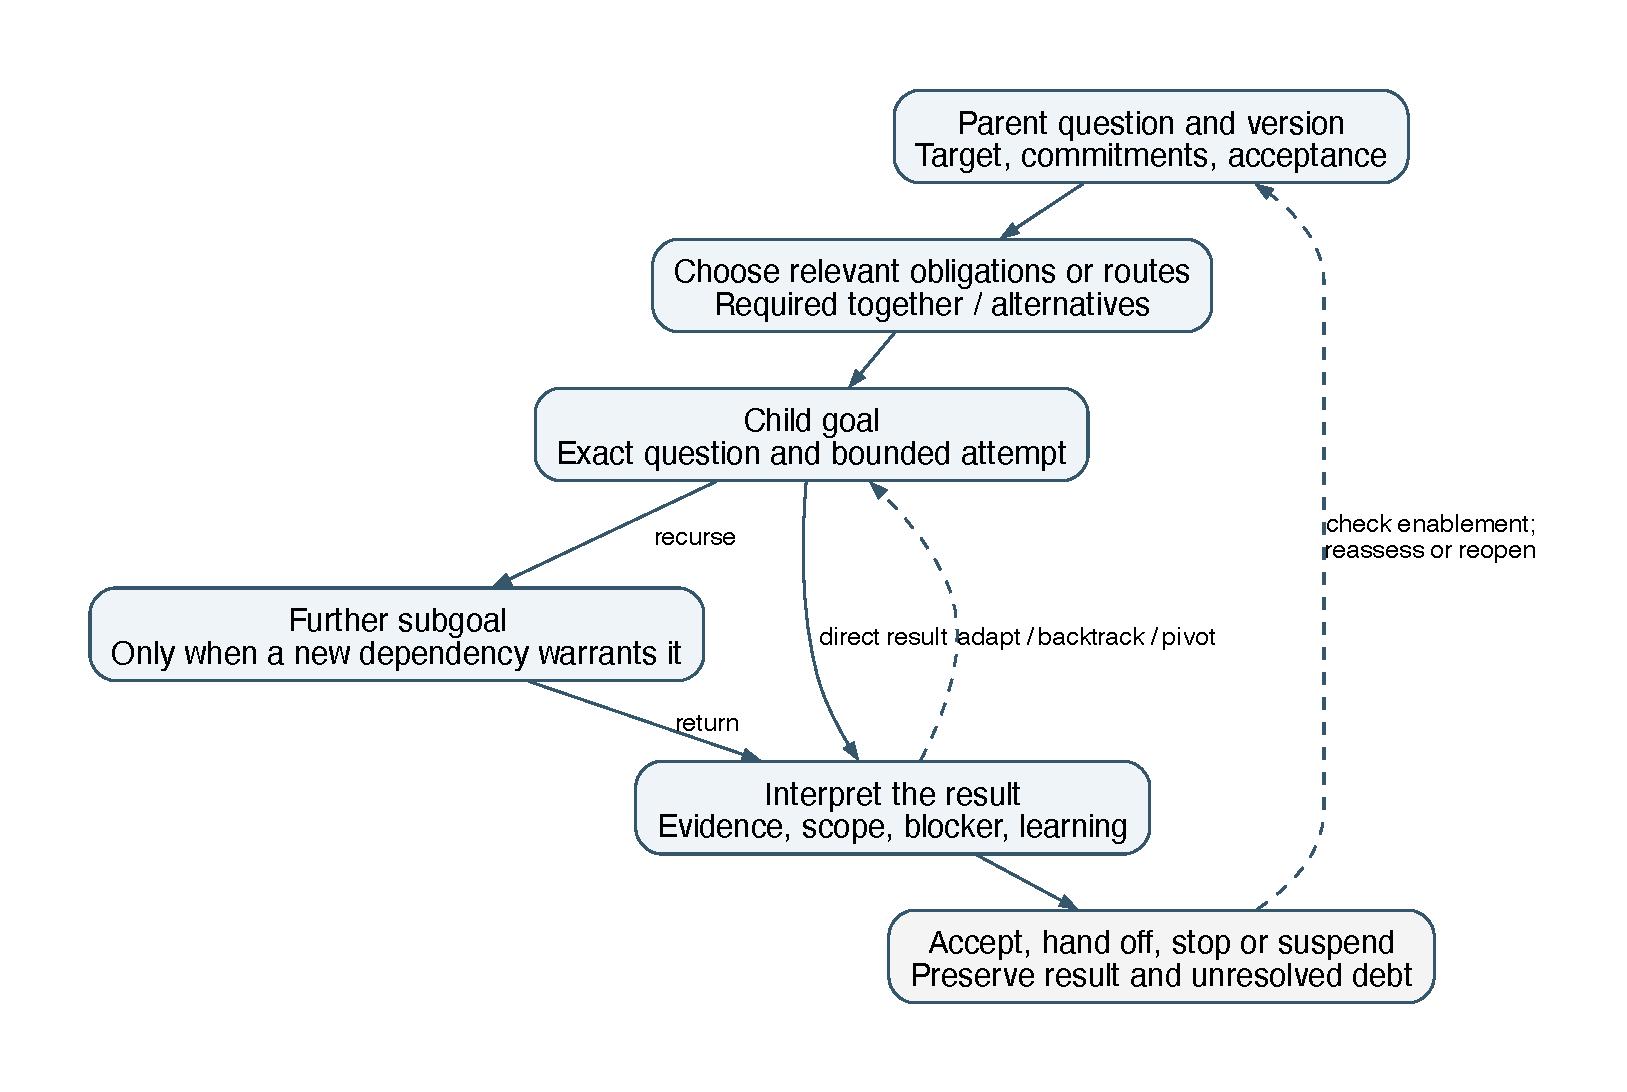
\includegraphics[width=.94\linewidth]{paper-workflow-representations/recursive-goals.pdf}
\caption{Recursive investigation as accountable decomposition and return.
The arrows express the management model in the text, not a recovered runtime
call graph. A child's report changes its parent's evidence and next decision;
it does not automatically mark that parent achieved.}
\label{fig:recursive-goals}
\end{figure}

\subsection{Decide whether to continue, change direction or stop}
A useful next attempt needs both a live connection to the target and a named
possible gain: discharge an obligation, discriminate alternatives, expose a
hidden premise, or make an explanation more precise. A failed attempt can justify
continuation when it supplies such information and changes the next move.
Repetition with unchanged inputs, the same blocker and no new learning needs a
control decision rather than another optimistic restatement.

\begin{table}[htbp]
\centering\small
\begin{tabularx}{\linewidth}{@{}>{\raggedright\arraybackslash}p{.17\linewidth}>{\raggedright\arraybackslash}X>{\raggedright\arraybackslash}X@{}}
\toprule
Decision & Criterion for the work & What returns to the parent \\
\midrule
Continue or adapt & Target remains relevant; the next bounded move has an explicit informative payoff & New attempt, changed formulation or discriminating check; goal remains open \\
Backtrack & An assumed premise, object identity or transfer has not been established & The missing prerequisite and the claims conditional on it \\
Pivot & The route repeatedly fails without useful new learning; a materially different route is justified & Preserved failure evidence and a new route, with no inherited proof status \\
Quarantine & Analogy, weaker scope or an unverified bridge prevents intended use & A retained result with restricted authority and conditions for rehabilitation \\
Stop or suspend & No target-relevant informative move is available, resources end, or a required dependency is unavailable & Terminal attempt or inactive branch; unresolved goal and reason remain recorded \\
Accept or hand off & The exact local acceptance criterion is met, or a bounded result is ready for its next validation stage & Scoped result, remaining debt and explicit parent-enablement check \\
\bottomrule
\end{tabularx}
\caption{An explanatory synthesis of source control distinctions. These are
work decisions, not a single scale of scientific confidence. Handoff and
resource exhaustion are especially distinct from proof.}
\label{tab:goal-stopping}
\end{table}

The stopping rule should be selected for the task rather than inferred from
how hard the problem feels. The contribution-oriented manager, for example,
prescribes at least two explicit adaptations or backtracks before stopping a
branch that still cannot name a contribution candidate, a disqualifying test or
a target-preserving validation handoff. This is a local contribution-search
policy, not a universal recursion depth or a guarantee that two attempts suffice.
The same source says not to stop solely because proof debt is hard. It also
requires broad exploration to end once a smallest defensible contribution has
reached its specified handoff boundary: validation and packaging then become
the appropriate work.\footnote{\path{skills/orchestration/contribution-oriented-subgoal-manager/SKILL.md},
``Good-Enough And Stop Policy.''}

Operational limits answer a different question: how much work may this attempt
consume? A recursion controller can allocate a finite total budget, cap depth
and live branches, charge children against the same budget, and require each
new expansion to identify what it adds. A stopped child must not acquire a
fresh unlimited allowance by being renamed or respawned. These are proposed
implementation disciplines for the explanatory model. Bounded expansion and
interruptible, bounded-duration actions can bound a run; a depth limit alone
cannot prevent unlimited sibling attempts, and none of these limits proves
scientific completeness or semantic convergence. Exhaustion returns ``unresolved
within this allocation,'' not ``false'' or ``impossible.''

\subsection{Return results, re-evaluate parents and reopen selectively}
The child returns a compact handoff:
\begin{description}[style=nextline,leftmargin=1.7cm,labelwidth=1.5cm,itemsep=1pt,parsep=0pt,topsep=4pt]
\item[Input] Exact parent requirement and goal version.
\item[Output] Result or failure; evidence, assumptions, scope and remaining debt.
\item[Check] Current context, required dependency and compatibility with sibling results.
\item[Next] Accept the supported contribution, revise the task or retain an unresolved obligation.
\end{description}
A lemma about the wrong carrier or a weaker quantifier can retain local value
without enabling parent closure.

If the parent changes its representation, premise or target, previously returned
children must be checked against that change. Some remain applicable, others
need translation or renewed work, and some become irrelevant to the revised
question. Historical results need not become false when their applicability
changes. Reopening follows the actual dependency chain: record the changed
assumption or evidence, the affected consumers, and a reason why renewed work
could now be informative. A late result for an old version is preserved and
reassessed; it is not silently attached to the current parent. Stopped or
quarantined branches can likewise reopen when a missing bridge, new source,
changed commitment or justified new allocation changes the decision conditions.
Renewed resources can resume unresolved work; they cannot rehabilitate a refuted
claim under unchanged assumptions. That requires a revised claim or context, or
evidence that defeats the purported counterexample.

\subsection{Two recursive levels in the running example}
Let the parent question be: can $q=x-y$ serve as a closed state description for
the stipulated dynamics? One child checks instantaneous observational adequacy;
another checks dynamical descent. These are joint requirements for this question.
The first child returns the already established quotient identification. The
second creates a further child: check whether $f(x,y)-g(x,y)$ is constant on each
fiber of $\pi$. It also retains the appropriate solution-existence obligations.

For $f=-x$ and $g=-y$, the fiber calculation gives $-q$, and the explicit flow
establishes descent. The result returns through the dynamical child to the
parent, which can accept this closed description for the stated linear model.
It does not thereby select an ontology for arbitrary physical systems.
For $f=x^2$ and $g=0$, the deeper child supplies the pair $(1,0),(2,1)$ with
unequal observable derivatives. The dynamical child returns a counterexample,
and the parent rejects closure under this particular combination of identity
and dynamics. The successful instantaneous child remains valid.

The next investigation can compare revised dynamics, a richer observable state,
or a revised redundancy claim. These are routes for a revised question, not
retroactive proofs of the failed original one. A shared invariance lemma can be
reused where its premises remain unchanged; an old linear-flow certificate
cannot certify the nonlinear model. If the available allocation ends before a
new route is justified, exploration stops with the incompatibility preserved
and the broader conceptual question open. This example shows why returning a
result is itself an act of interpretation: the same subsidiary failure closes
one precise claim while opening a more informative parent-level inquiry.

\section{How the workflows form a research process}
\label{sec:workflow-relationships}
A workflow supplies a reusable procedure for a particular research need; its
invocation is an attempt to advance a goal. Several workflows can serve one goal,
and the same workflow can serve different goals at different recursive depths. The
relationship among workflows is therefore explained by the question passed in,
the change produced, and the decision that can use it. It is not a universal
pipeline in which every investigation executes all nineteen workflows.
Figure~\ref{fig:workflow-ecosystem} gives a grouped reading map;
Appendix~\ref{app:workflow-relationships} identifies every scoped workflow and
its specific incoming and outgoing role.

Four kinds of connection must be distinguished. Native occurrences declare
artifact dependencies \emph{within} a flow. Source reasoning policies may
prescribe a switch to another named workflow while the native declaration only
returns a disposition. The Cohere registry additionally declares a parent with
five ordered subworkflows. An editorial connection means that a result would
be relevant to another workflow; it is not evidence that an adapter or automatic
invocation exists. Our overview labels these differences instead of turning
plausible research relationships into runtime claims.

\begin{figure}[htbp]
\centering
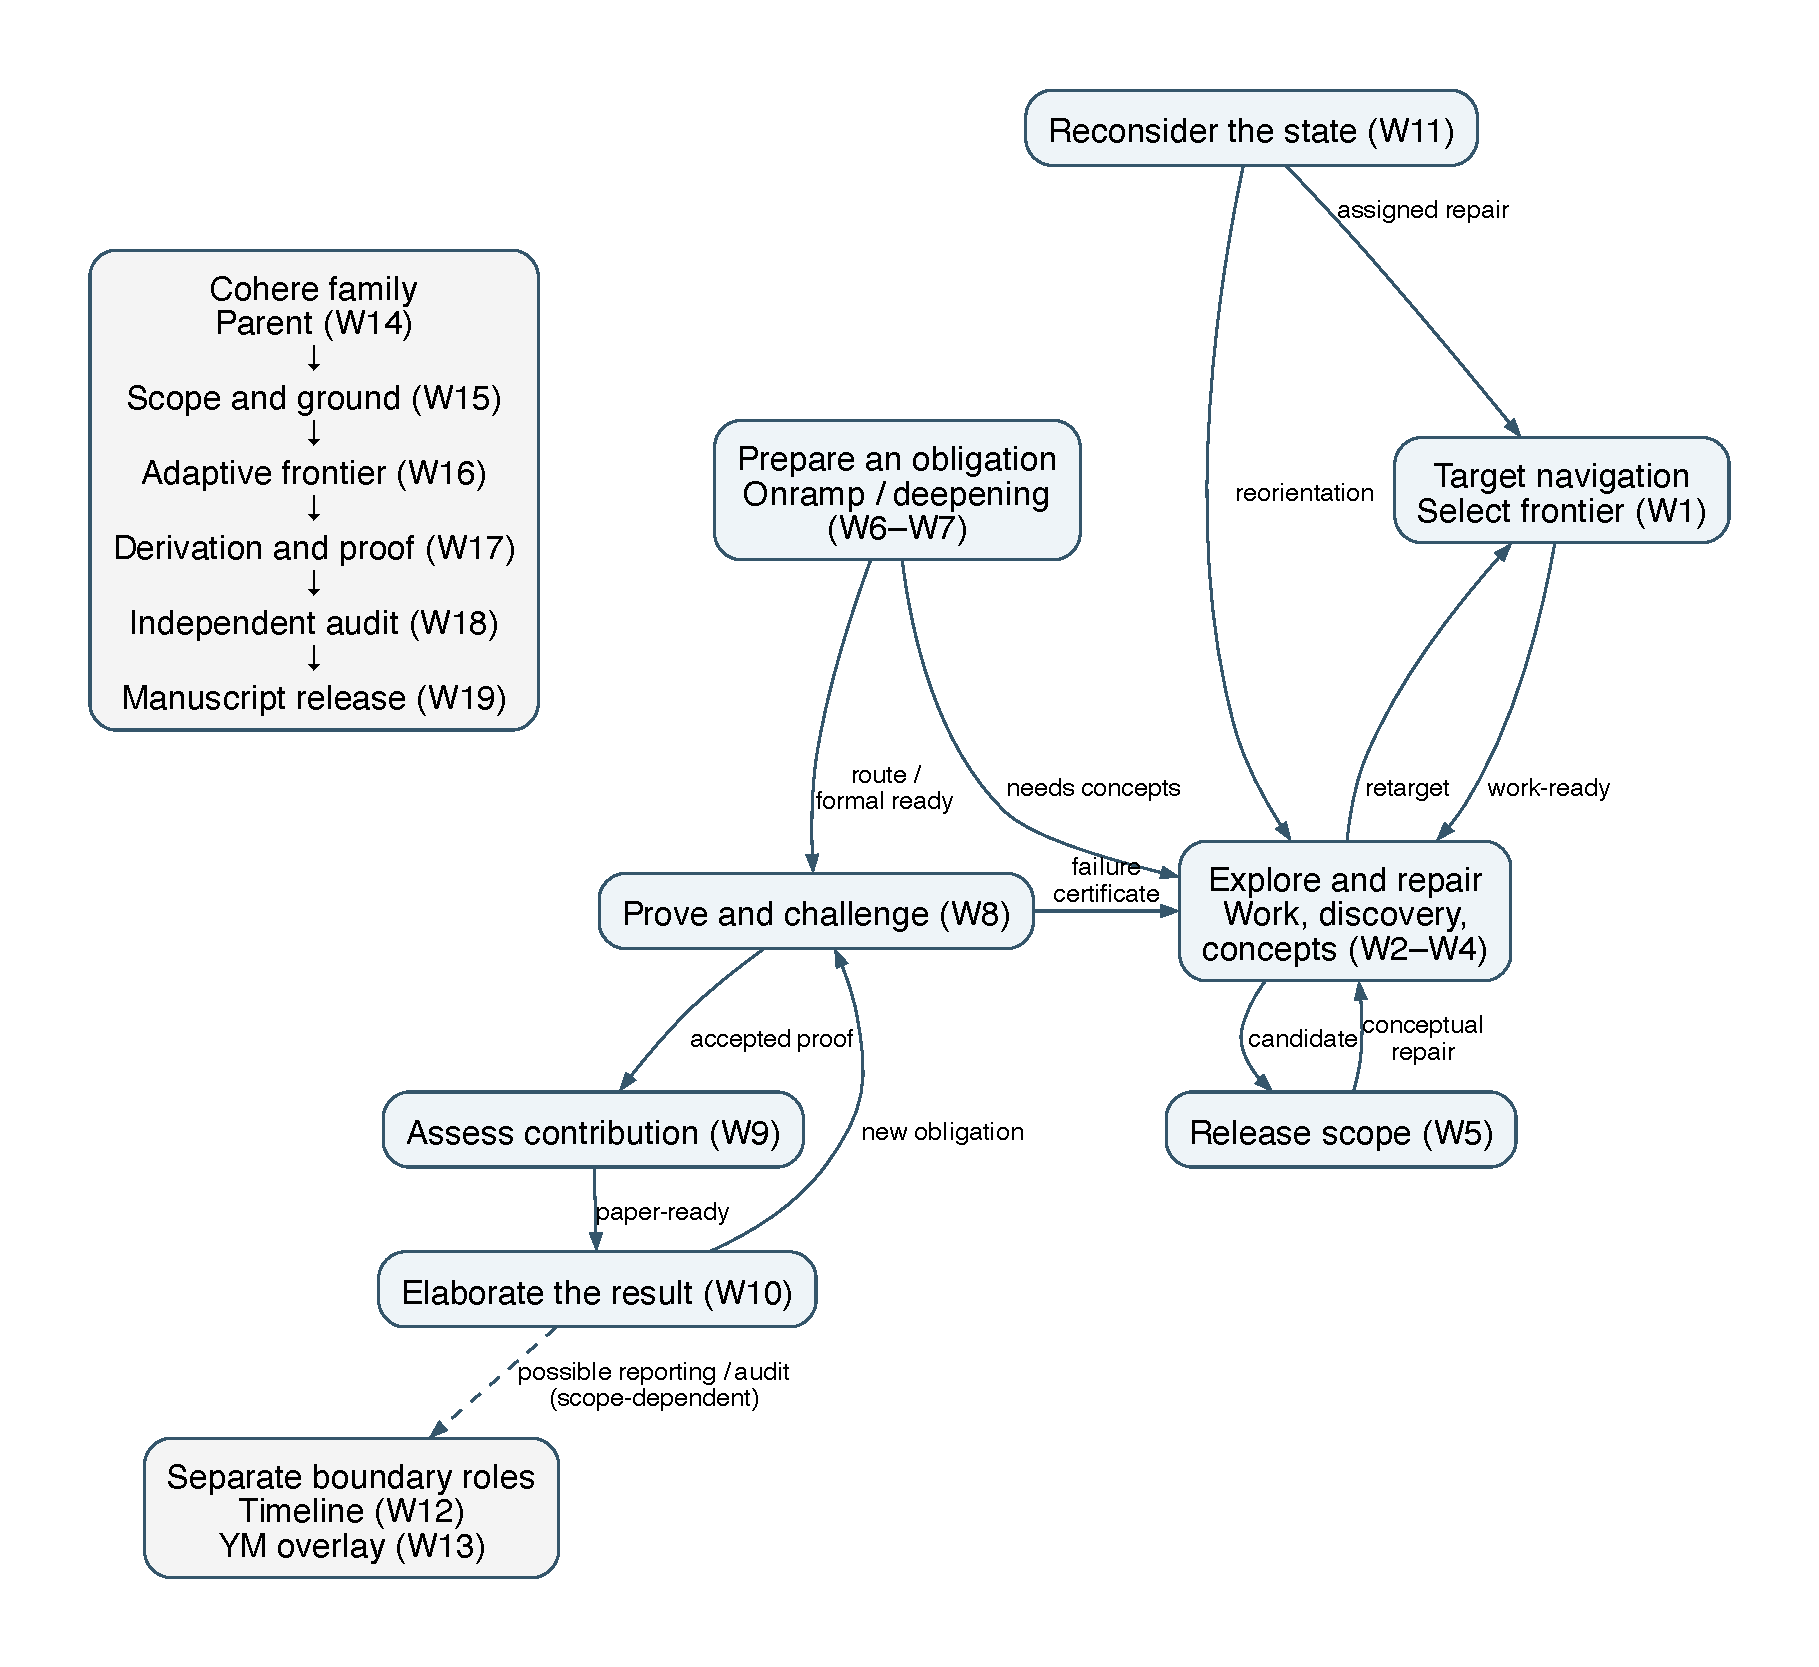
\includegraphics[width=\linewidth]{paper-workflow-representations/workflow-ecosystem.pdf}
\caption{A grouped map of research roles. Solid arrows summarize prescribed
routing between selected members of the grouped workflow families, not all
member-to-member connections or every declared edge; dashed arrows denote editorial
feedback or applicability, requiring an explicit handoff. The separate Cohere
box has declared internal subworkflow composition, but no general-discovery
entry edge is asserted. Exact workflow names and source qualifications appear
in Appendix~\ref{app:workflow-relationships}.}
\label{fig:workflow-ecosystem}
\end{figure}

\paragraph{Orient and explore.}
Target navigation identifies which unresolved obligation deserves the next
allocation. A focused abductive loop can address a bounded explanatory gap;
a discovery marathon coordinates a wider portfolio. Conceptual hypothesis
exploration and conceptual frontier deepening address failures of the inherited
representation and mature alternatives through reflection. Their contribution
is to make a better question or candidate available, with its protected
successes, objections and burdens. A diagnostic no-preference outcome returns
for revision; it does not itself authorize a preferred proof route.

\paragraph{Turn a mature question into support.}
The evidence-to-proof onramp develops a route from an evidence-bearing candidate;
theorem proof delivery addresses an exact theorem and its closure conditions.
These can become children of a conceptual programme when the programme has
produced the necessary question and the source gates permit the handoff.
A proof result answers its exact obligation. A failed transfer or unresolved
premise returns a blocker that can motivate route revision or conceptual
reconsideration, with the broader return connection made explicit by the caller.

\paragraph{Reconsider and consolidate.}
Deep review and reorientation examines the current reasoning state and can
produce a corrective agenda. Scientific contribution cultivation asks whether
a result has a defensible independent payoff; manuscript result elaboration
explicates its actual consequences and remaining limits. Release promotion
judges whether the relevant evidence and gates support a release disposition.
These activities have different acceptance conditions: a coherent exposition,
a worthwhile contribution, a proved theorem and a release decision are not
interchangeable achievements.

\paragraph{Keep special compositions and overlays in scope.}
Cohere is a separately declared parent workflow whose children scope and ground,
explore an adaptive frontier, derive and prove, independently audit, and prepare
manuscript release. Its structure supplies a concrete example of nested work,
but unresolved native producers remain projection gaps. The timeline-paper
workflow independently reports a bounded research history; it does not confer
proof authority. The Yang--Mills representational-dynamics overlay attaches
domain-specific representational checks to an applicable inquiry. Neither its
name nor its inclusion makes a result a Yang--Mills theorem. These boundary
roles should be attached only where their input and scope requirements fit.

Across these families, recursive goal records provide a common \emph{handoff
interpretation}: identify the parent question, the requested contribution, the
accepted evidence and the conditions for returning or stopping. They do not
supply missing executable wiring. A workflow can discharge a subgoal, create
new children, recommend another route, or return a reason to stop. The parent
retains responsibility for interpreting that outcome against the scientific
question that made the invocation worthwhile.


\section{Inferential operations and Prism as supporting descriptions}
\label{sec:conceptual-support}
Abduction, deduction, induction, transfer, contrast, refutation and calibration
remain useful distinctions. They answer how a local commitment is proposed,
extended, challenged or assessed. They do not determine which conceptual tension
matters or what a new representation should mean. The correspondence is
many-to-many: one conceptual transformation can need several operations, and the
same operation can contribute to several different conceptual tasks.

\begin{table}[htbp]
\centering\small
\begin{tabularx}{\linewidth}{@{}>{\raggedright\arraybackslash}p{.30\linewidth}>{\raggedright\arraybackslash}X>{\raggedright\arraybackslash}X@{}}
\toprule
Conceptual task & Possible inferential work & What the type alone leaves open \\
\midrule
Locate a pressure & Compare cases, derive a conflict, test a claim & Which commitment creates the difficulty \\
Diagnose the bottleneck & Contrast explanations, reconstruct assumptions, assess evidence & Whether concepts or ordinary work need changing \\
Construct a mediator & Propose an object, map structures, derive constraints & Why the object resolves this pressure and preserves successes \\
Reflect on identity & Reconstruct a candidate, develop its strongest objection, revise & Which distinction changes and what it now explains \\
Develop a programme & Articulate consequences, seek defeaters, compare rivals & Which question is now worth pursuing and why \\
\bottomrule
\end{tabularx}
\caption{Illustrative relationships, not exclusive assignments or a required
operation sequence. Inference labels annotate conceptual work rather than replace
its explanation.}
\label{tab:conceptual-inference-map}
\end{table}

In the example, quotient construction can be described as a proposed mediator,
its observable invariance can be checked deductively, and the incompatible
dynamics supplies a refutational counterexample. These classifications do not
explain the initial mismatch between raw coordinate identity and the target's
observable identity. That explanation depends on the reconstructed situation.

Prism adds a further discipline: state which artifact is consumed, which
candidate a finding concerns, which context must be retained, and what relation
licenses a transition. An assessment of the compatible linear dynamics cannot
be silently reused for the nonlinear candidate. A typed join makes the intended
dependency visible, although nominal types do not by themselves guarantee semantic
identity or scientific correctness. Unresolved producers and absent adapters
must remain visible rather than being filled with an imagined execution.

The supporting calculus in Appendix~\ref{app:supporting-calculus} provides local
inference notation, motifs and control abstractions. Its status-only calibration
operator is a deliberately narrow abstraction; substantive interpretation and
reconstruction during comparison can produce new conceptual content and need
their own account. Similarly, expressing reflection with familiar operation types
is a representational possibility, not an explanation of what makes reflection
productive. Appendix~\ref{app:granular-prism-workflows} retains the complete native
occurrence descriptions and worked cases at that lower level.

\section{Evidence, limitations and implications for system design}
\label{sec:conceptual-evidence}
The evidence for this paper is local source material: conceptual-discovery
instructions, related reflection and bridge procedures, and the nineteen native
workflow declarations with their linked procedure accounts, together with
subgoal control, result-memory and enablement policies. The recursive goal graph,
shared-budget discipline and proposed handback semantics are an explanatory
management model, not a verified universal runtime. The main narrative
is an interpretive synthesis of those sources. The tension distinctions and
the pair-state example are authorial explanatory constructions. They are not
reported executions, discovered physical mechanisms or empirical comparisons.

The sources are not one uniform protocol. The conceptual-frontier profile makes
six reflection transformations explicit; broader reflective discovery selects
applicable lenses and permits a nonconceptual exit. Native workflows can omit
procedural detail, routing effects or producers specified elsewhere. The
appendices preserve these differences. A common conceptual description must not
be mistaken for proof that those layers are behaviorally equivalent.

The account suggests that an inquiry-support system should retain more than a
candidate and its status. It should preserve the pressure being addressed, the
incumbent successes, the distinctions changed, the strongest objection, and the
new burden that follows. Comparison should read complete conceptual content;
it should preserve unresolved differences and allow no justified preference.
Formalization should expose a specific obligation, while proof, symbolic work
or measurement should answer a question that the theory has made precise.

These are design implications, not measured benefits. Evaluating them would
require evidence beyond successful generation or complete paperwork: whether
the proposed tension is real, whether a transformation changes the underlying
concepts, whether it preserves required successes, and whether the resulting
question is useful. Neither a rich vocabulary nor a passing type check answers
those questions. This paper does not establish novelty, comparative discovery
performance, universal cognitive stages, or any Yang--Mills theorem. The
domain-specific appendix remains a set of explicitly conditional examples.

\section{Conclusion}
Scientific inquiry can advance by changing what its questions are about. A
localized tension reveals which commitment is under pressure; diagnosis separates
conceptual defects from ordinary unfinished work; alternative construction changes
objects, distinctions or explanatory relations; and reflection exposes the
preservation conditions and objections those changes create. A useful outcome may
be a better representation, a sharper incompatibility, a plural set of programmes,
or a newly explicit proof obligation.

The organizing unit is therefore the transformation of a conceptual situation.
Inferential categories describe constituent moves, and Prism interfaces make
their dependencies inspectable. Recursive goal management preserves the parent
question through decomposition, bounded attempts and evidence-sensitive returns.
Stopping a branch leaves its scientific status explicit; a workflow handoff
changes what may be attempted next without automatically closing a parent.
The workflow map connects these roles while preserving the distinction between
source-prescribed switches and editorial coordination. In the worked example, the decisive change is
from raw coordinate difference to observable-state identity, followed by the
recognition that dynamics must respect that identity. The formal checks become
informative because the conceptual question has been made precise. Preserving
that relationship between tension, transformation and remaining burden gives the
reasoning account its explanatory content.
